\begin{flushleft}

\subsection{Sekvensdiagram}
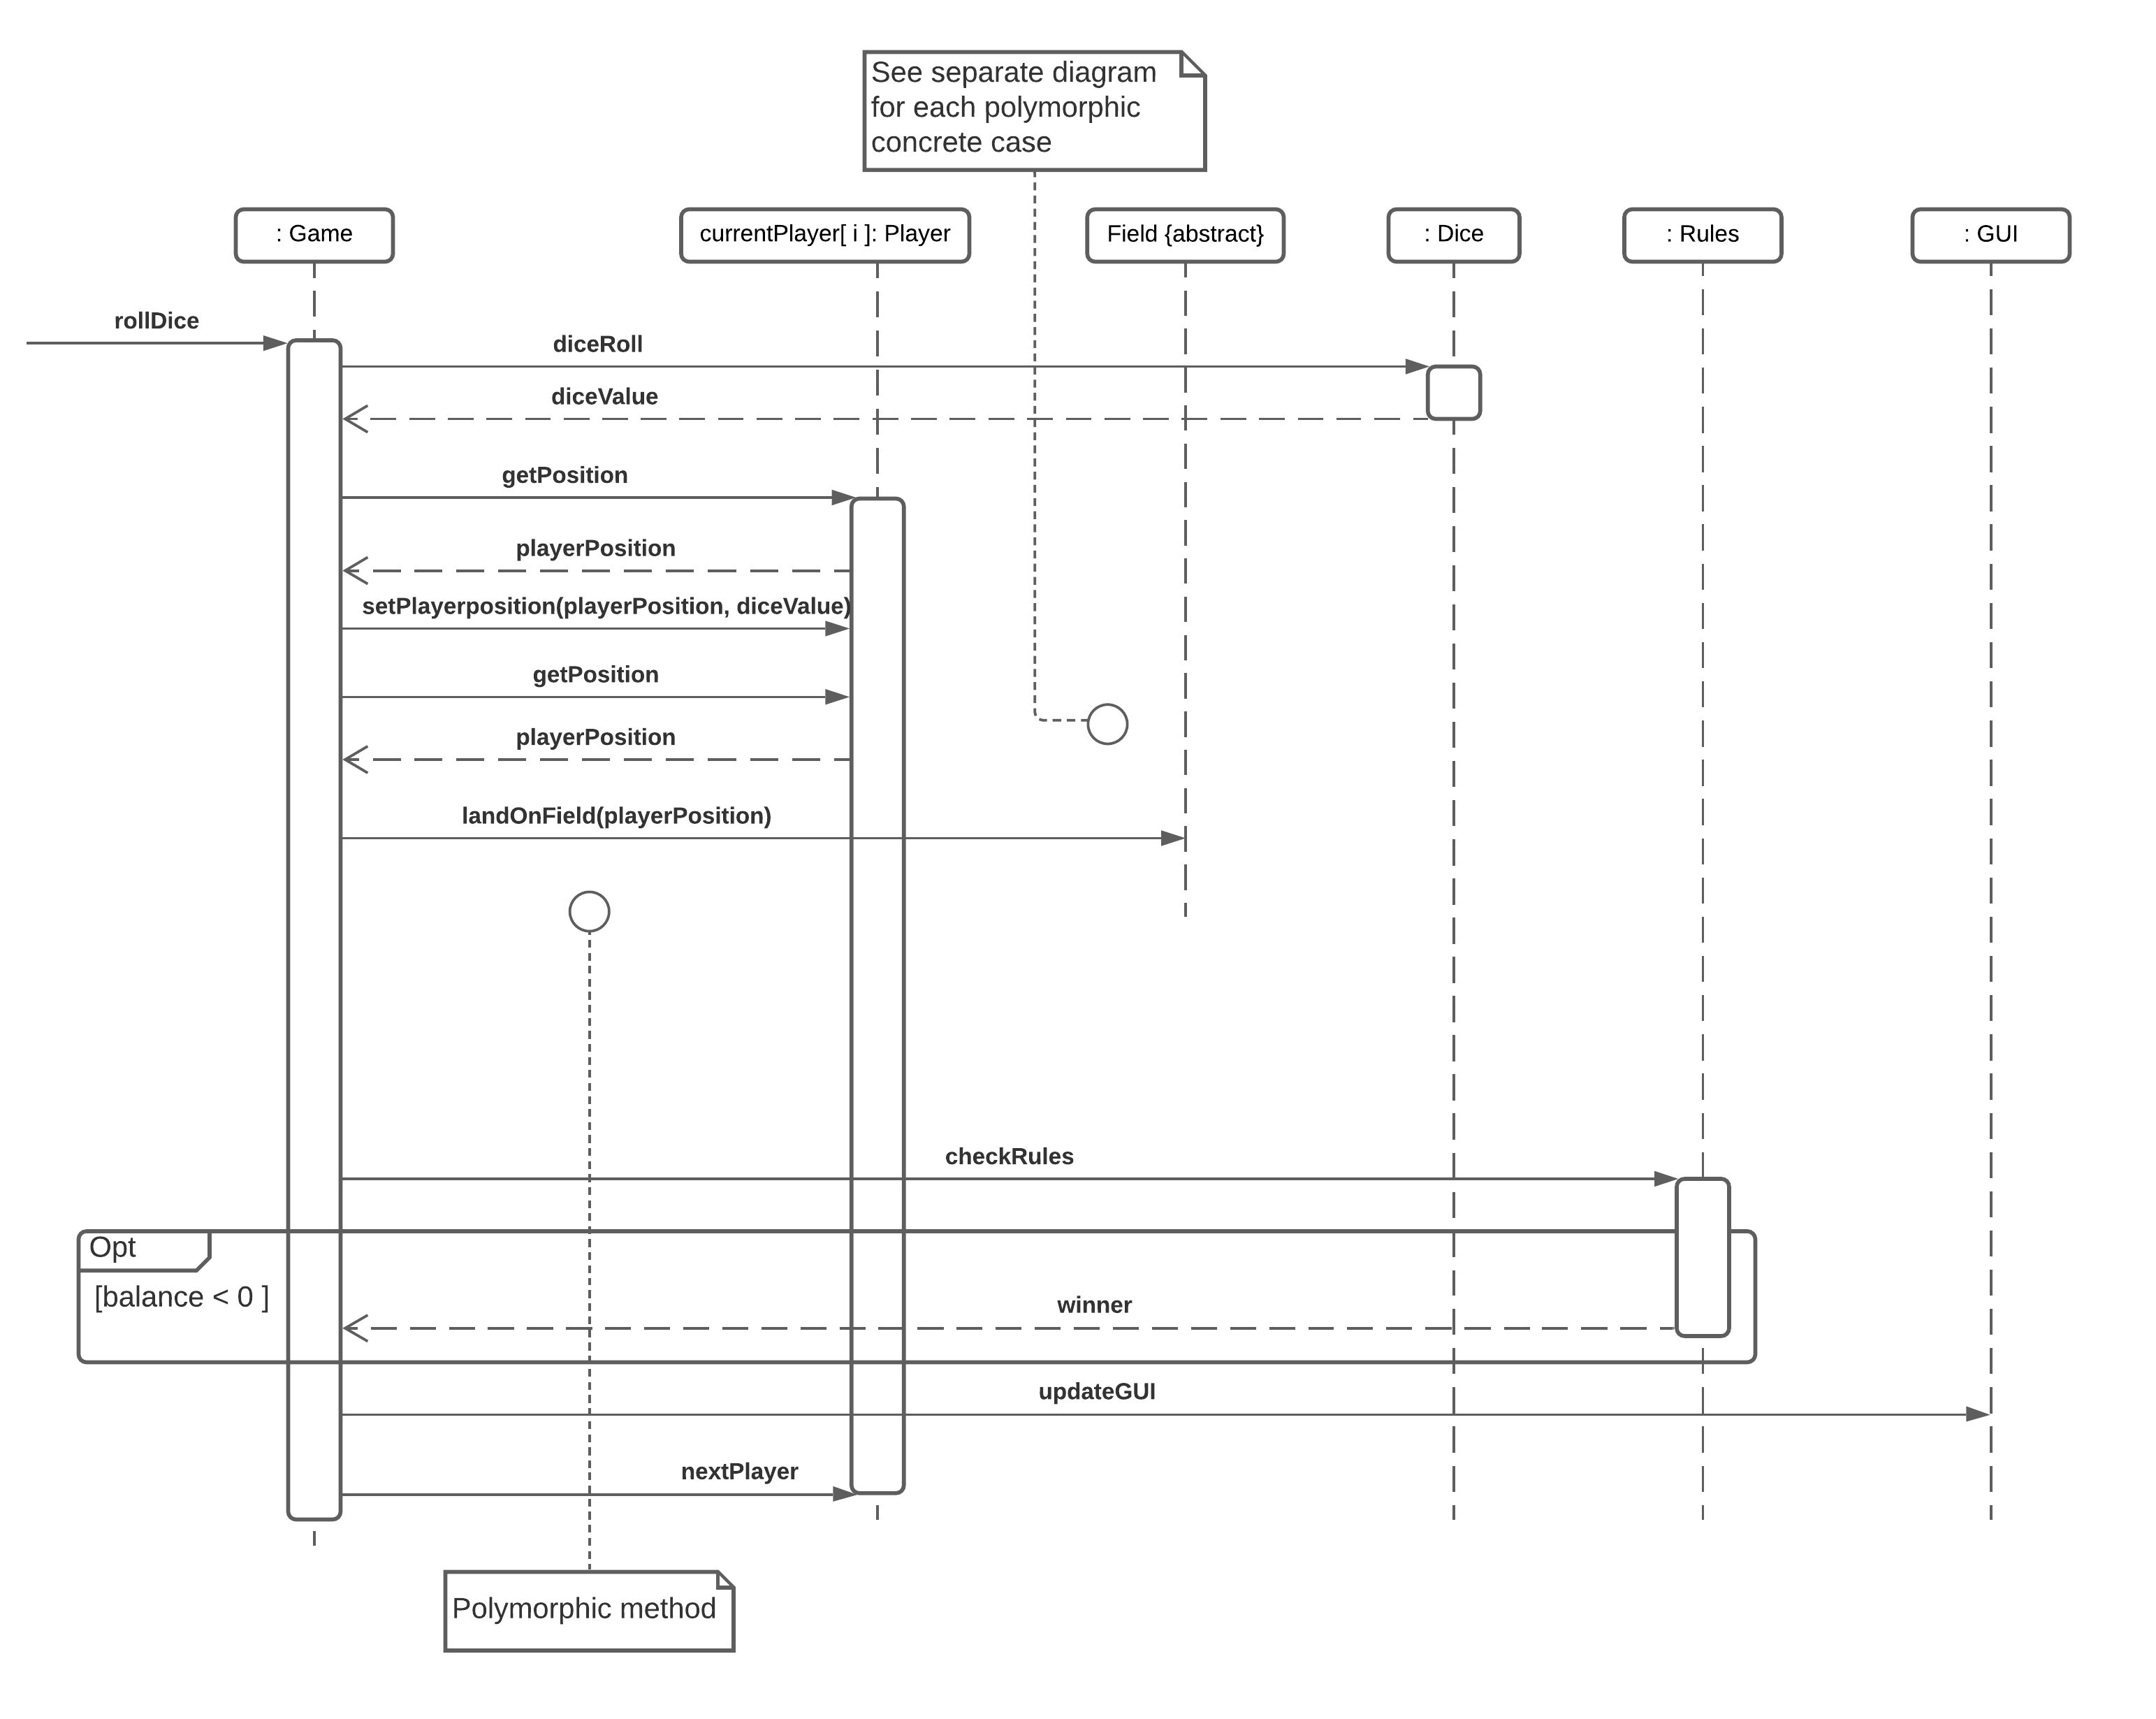
\includegraphics[width=0.9\textwidth]{Report/figures/Sekvensdiagram1.png}~\\[1cm]
Figur 5.1.1. Sekvensdiagram over rollDice som use-case.

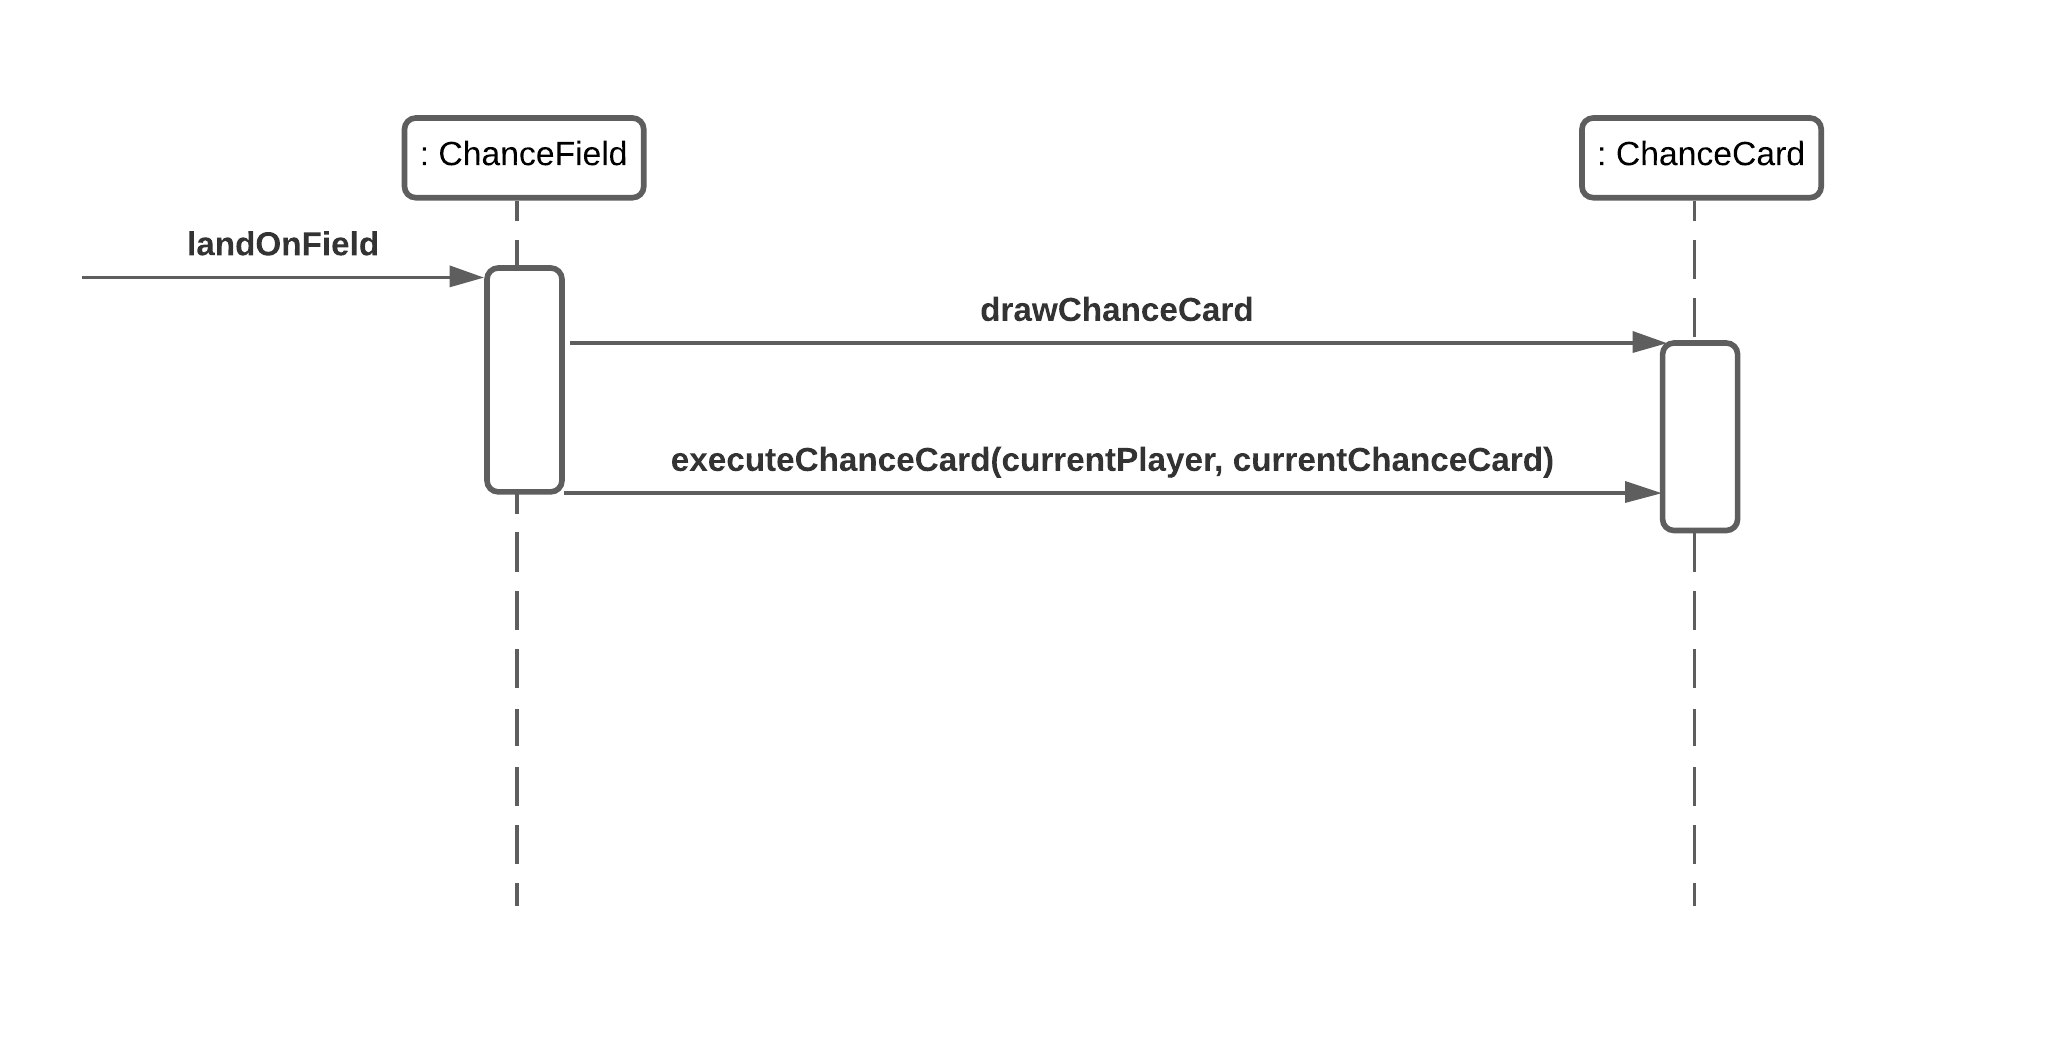
\includegraphics[width=0.9\textwidth]{Report/figures/Sekvensdiagram_ChanceField.png}~\\[1cm]
Figur 5.1.2. Sekvensdiagram over polymorphism af metoden landOnField for ChanceField.


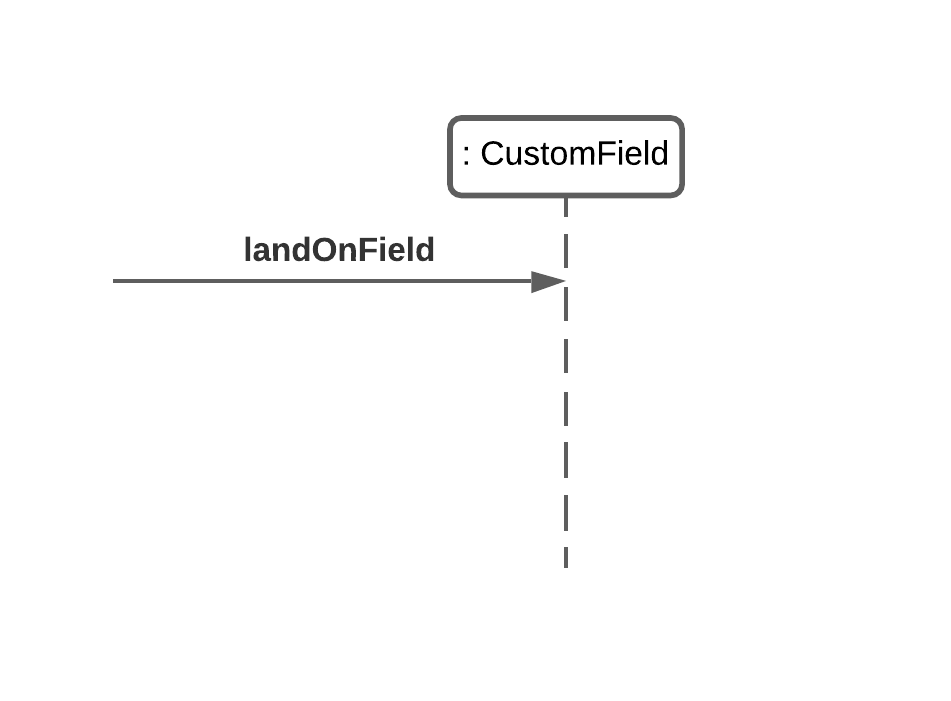
\includegraphics[width=0.9\textwidth]{Report/figures/Sekvensdiagram_CustomField.png}~\\[1cm]
Figur 5.1.3. Sekvensdiagram over polymorphism af metoden landOnField for CustomField.


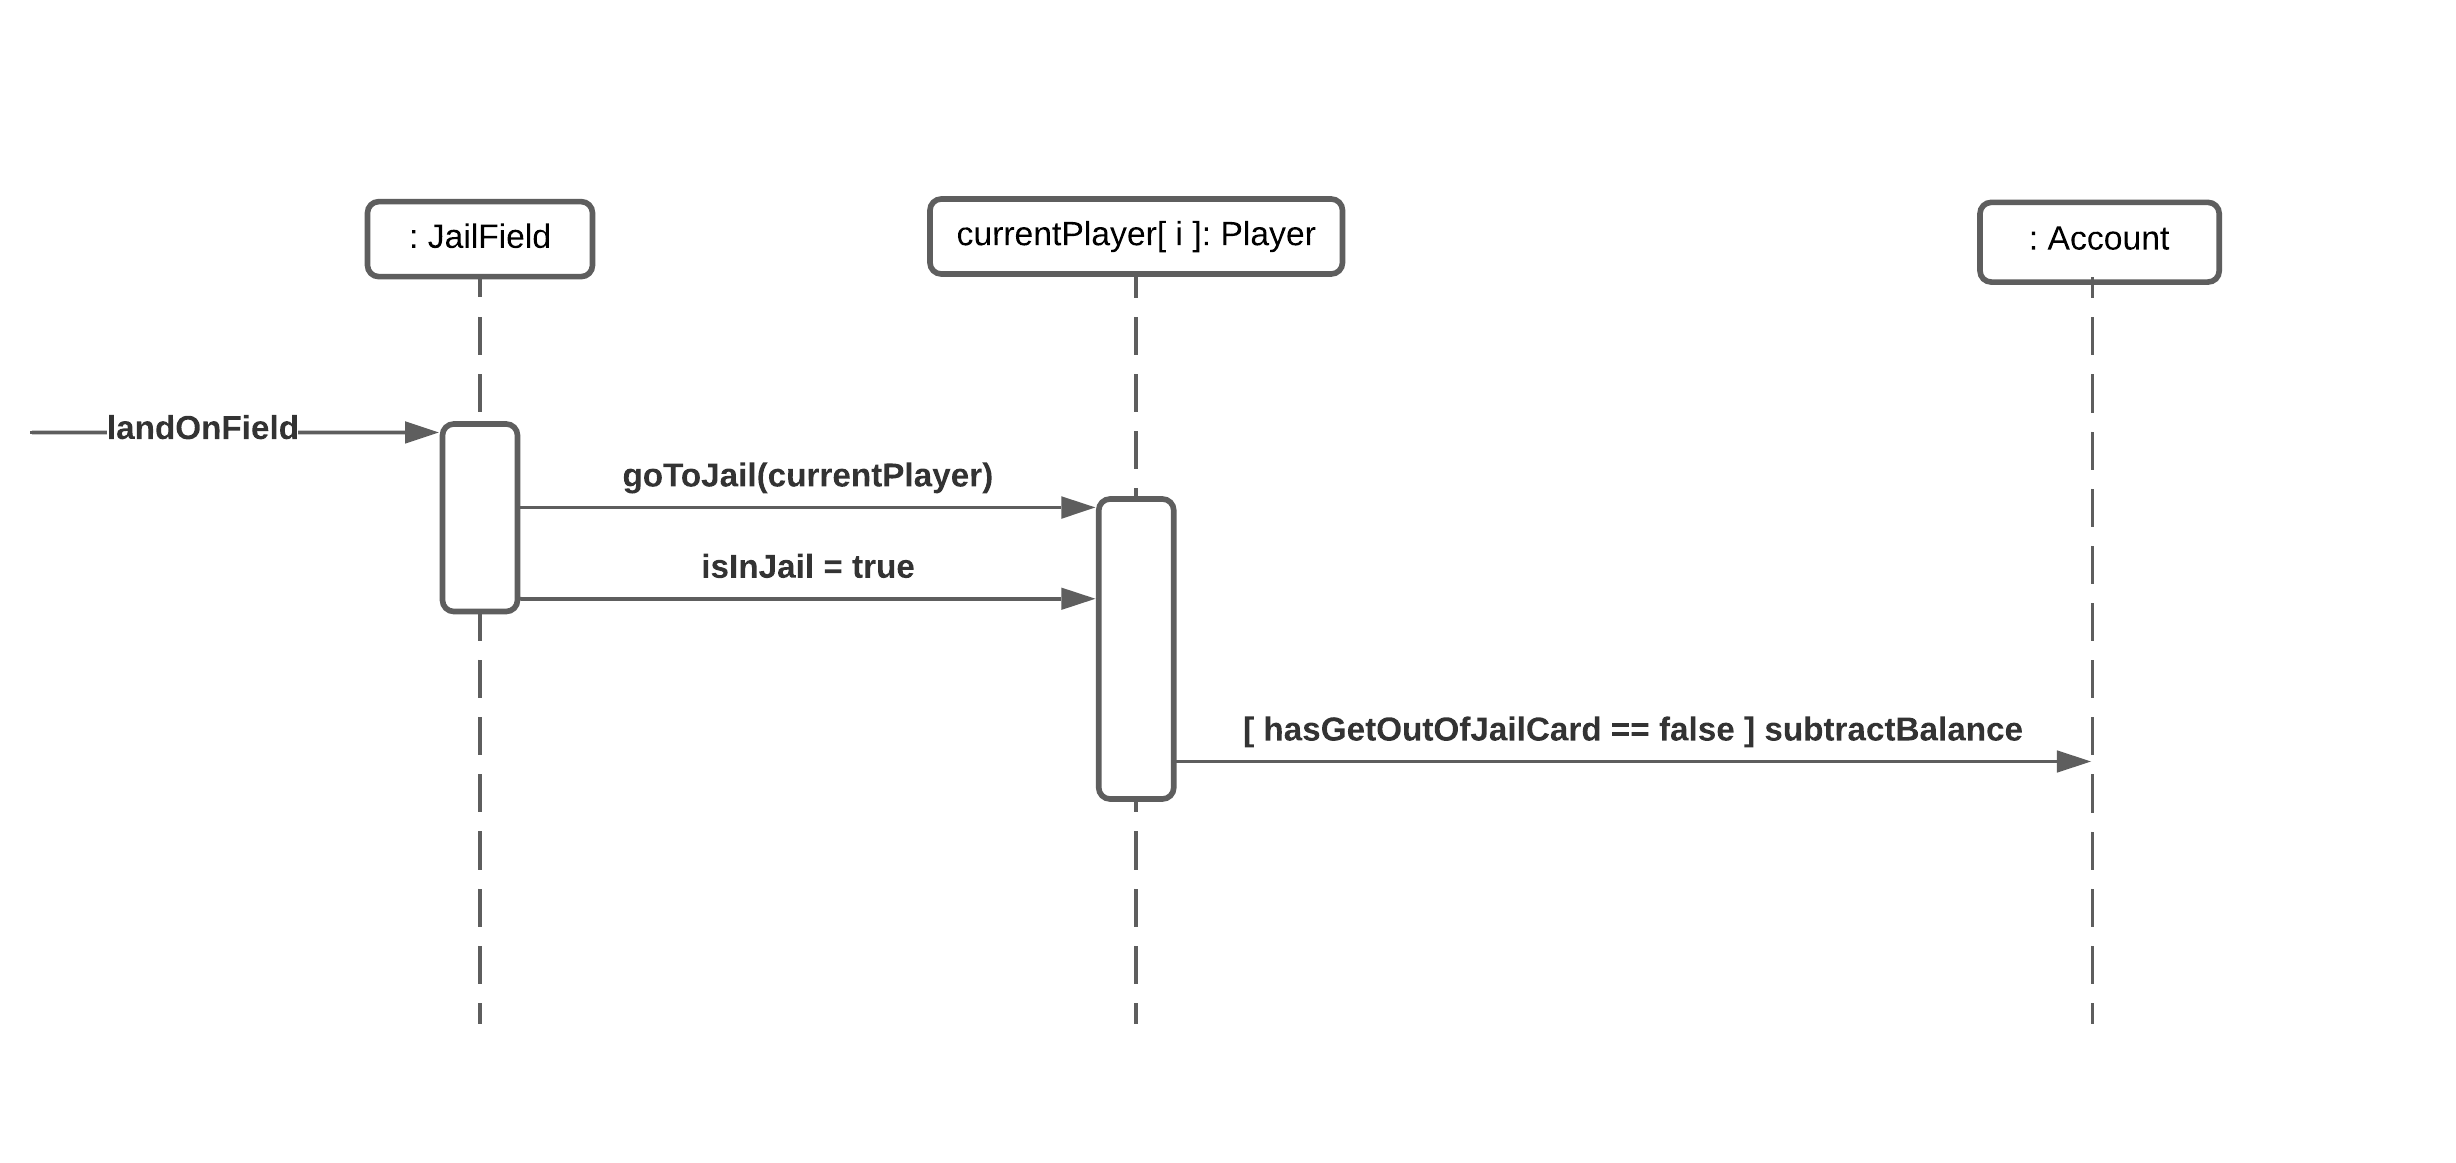
\includegraphics[width=0.9\textwidth]{Report/figures/Sekvensdiagram_JailField.png}~\\[1cm]
Figur 5.1.4. Sekvensdiagram over polymorphism af metoden landOnField for JailField.


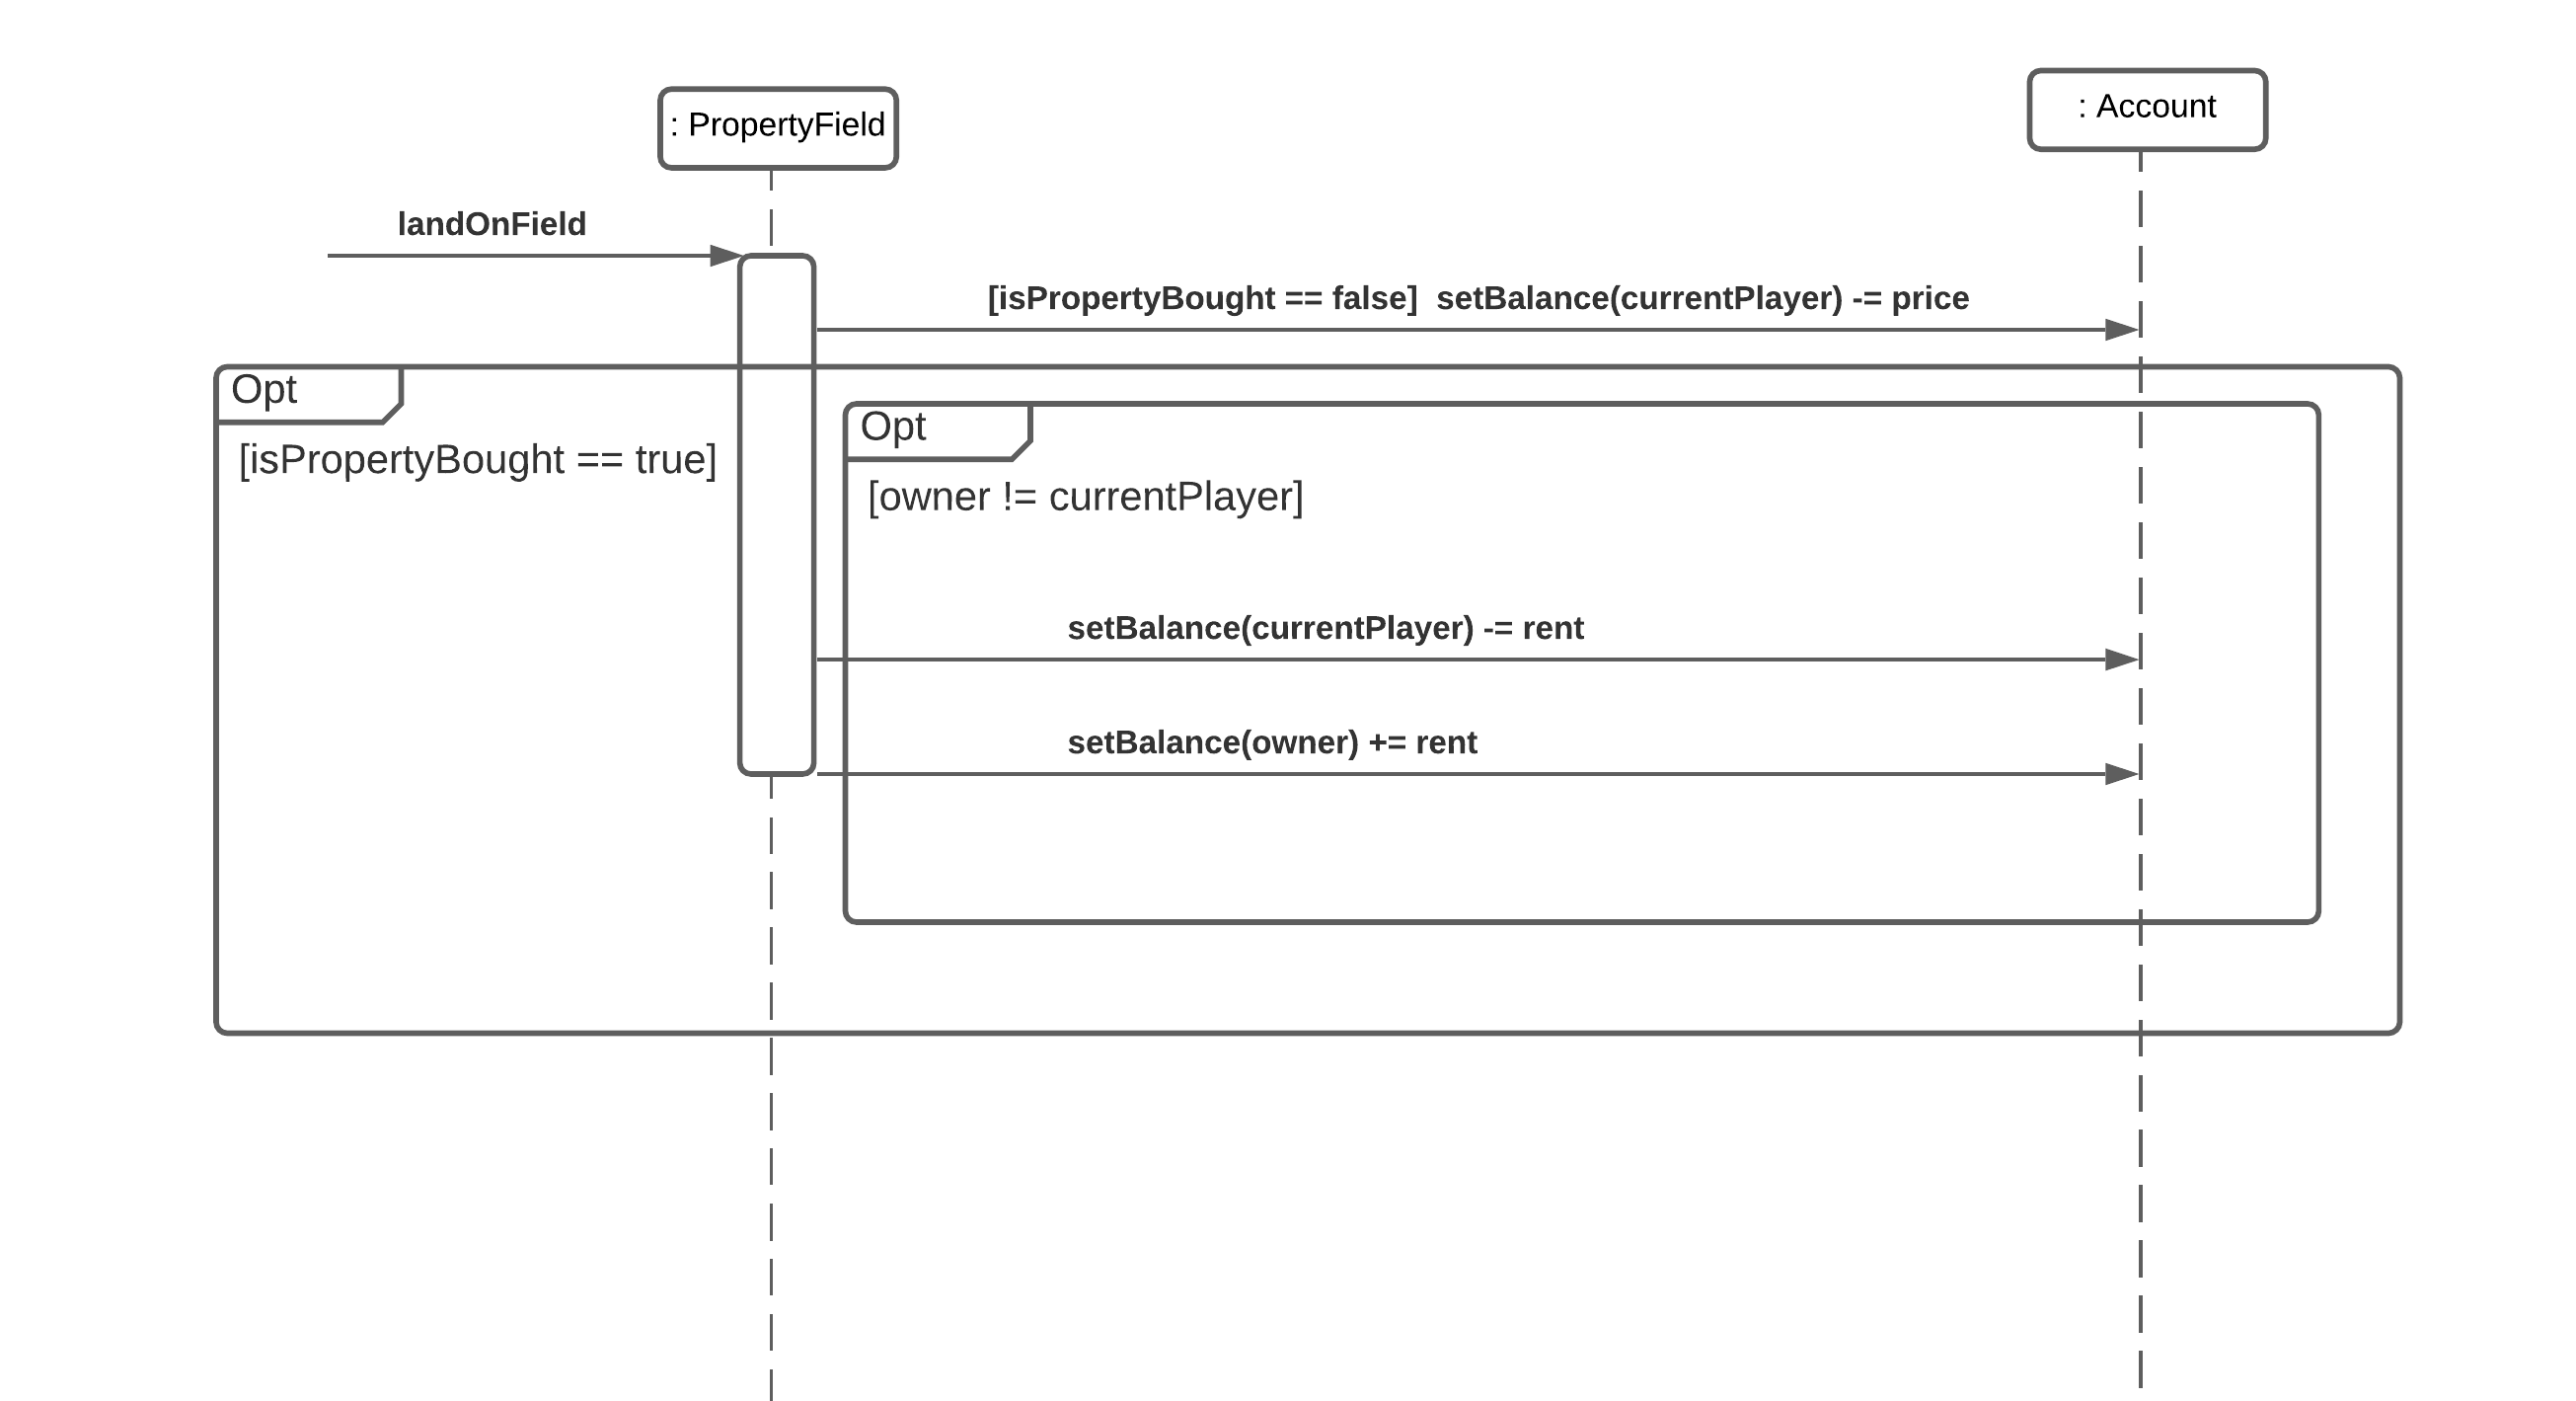
\includegraphics[width=0.9\textwidth]{Report/figures/Sekvensdiagram_PropertyField.png}~\\[1cm]
Figur 5.1.5. Sekvensdiagram over polymorphism af metoden landOnField for PropertyField.


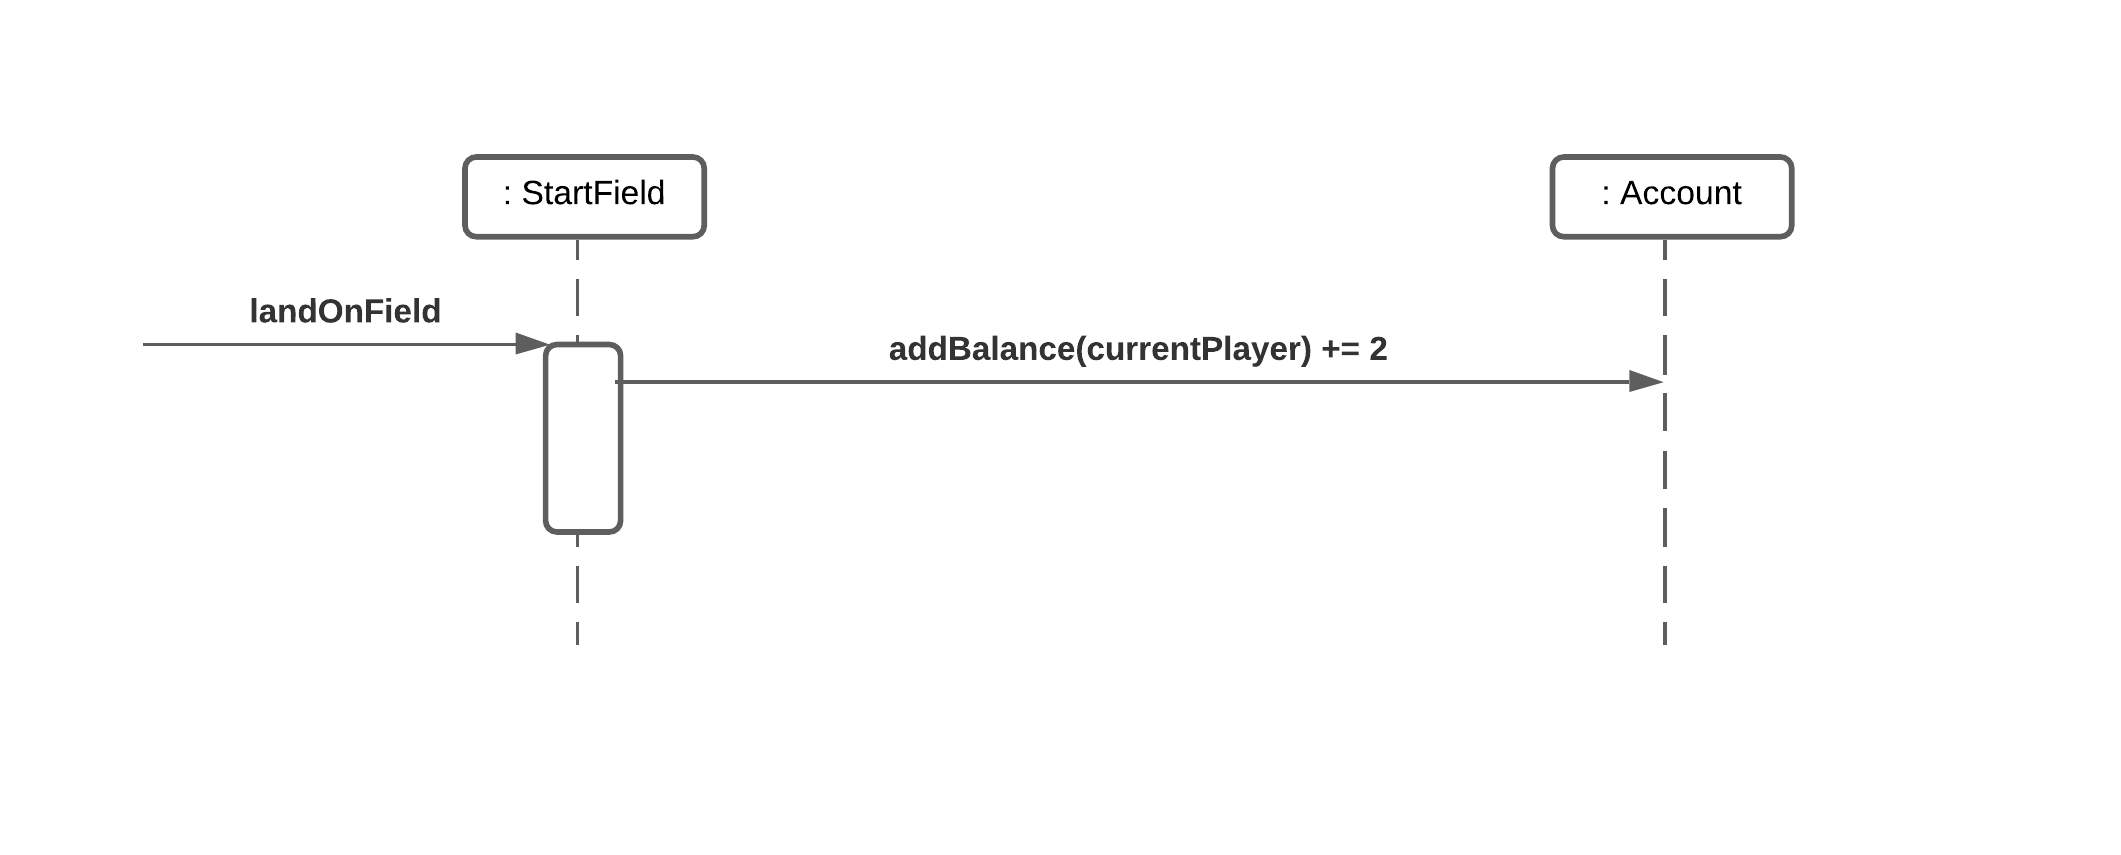
\includegraphics[width=0.9\textwidth]{Report/figures/Sekvensdiagram_StartField.png}~\\[1cm]
Figur 5.1.6. StartField over polymorphism af metoden landOnField for ChanceField..





\subsection{Designklassediagram}
\begin{center}
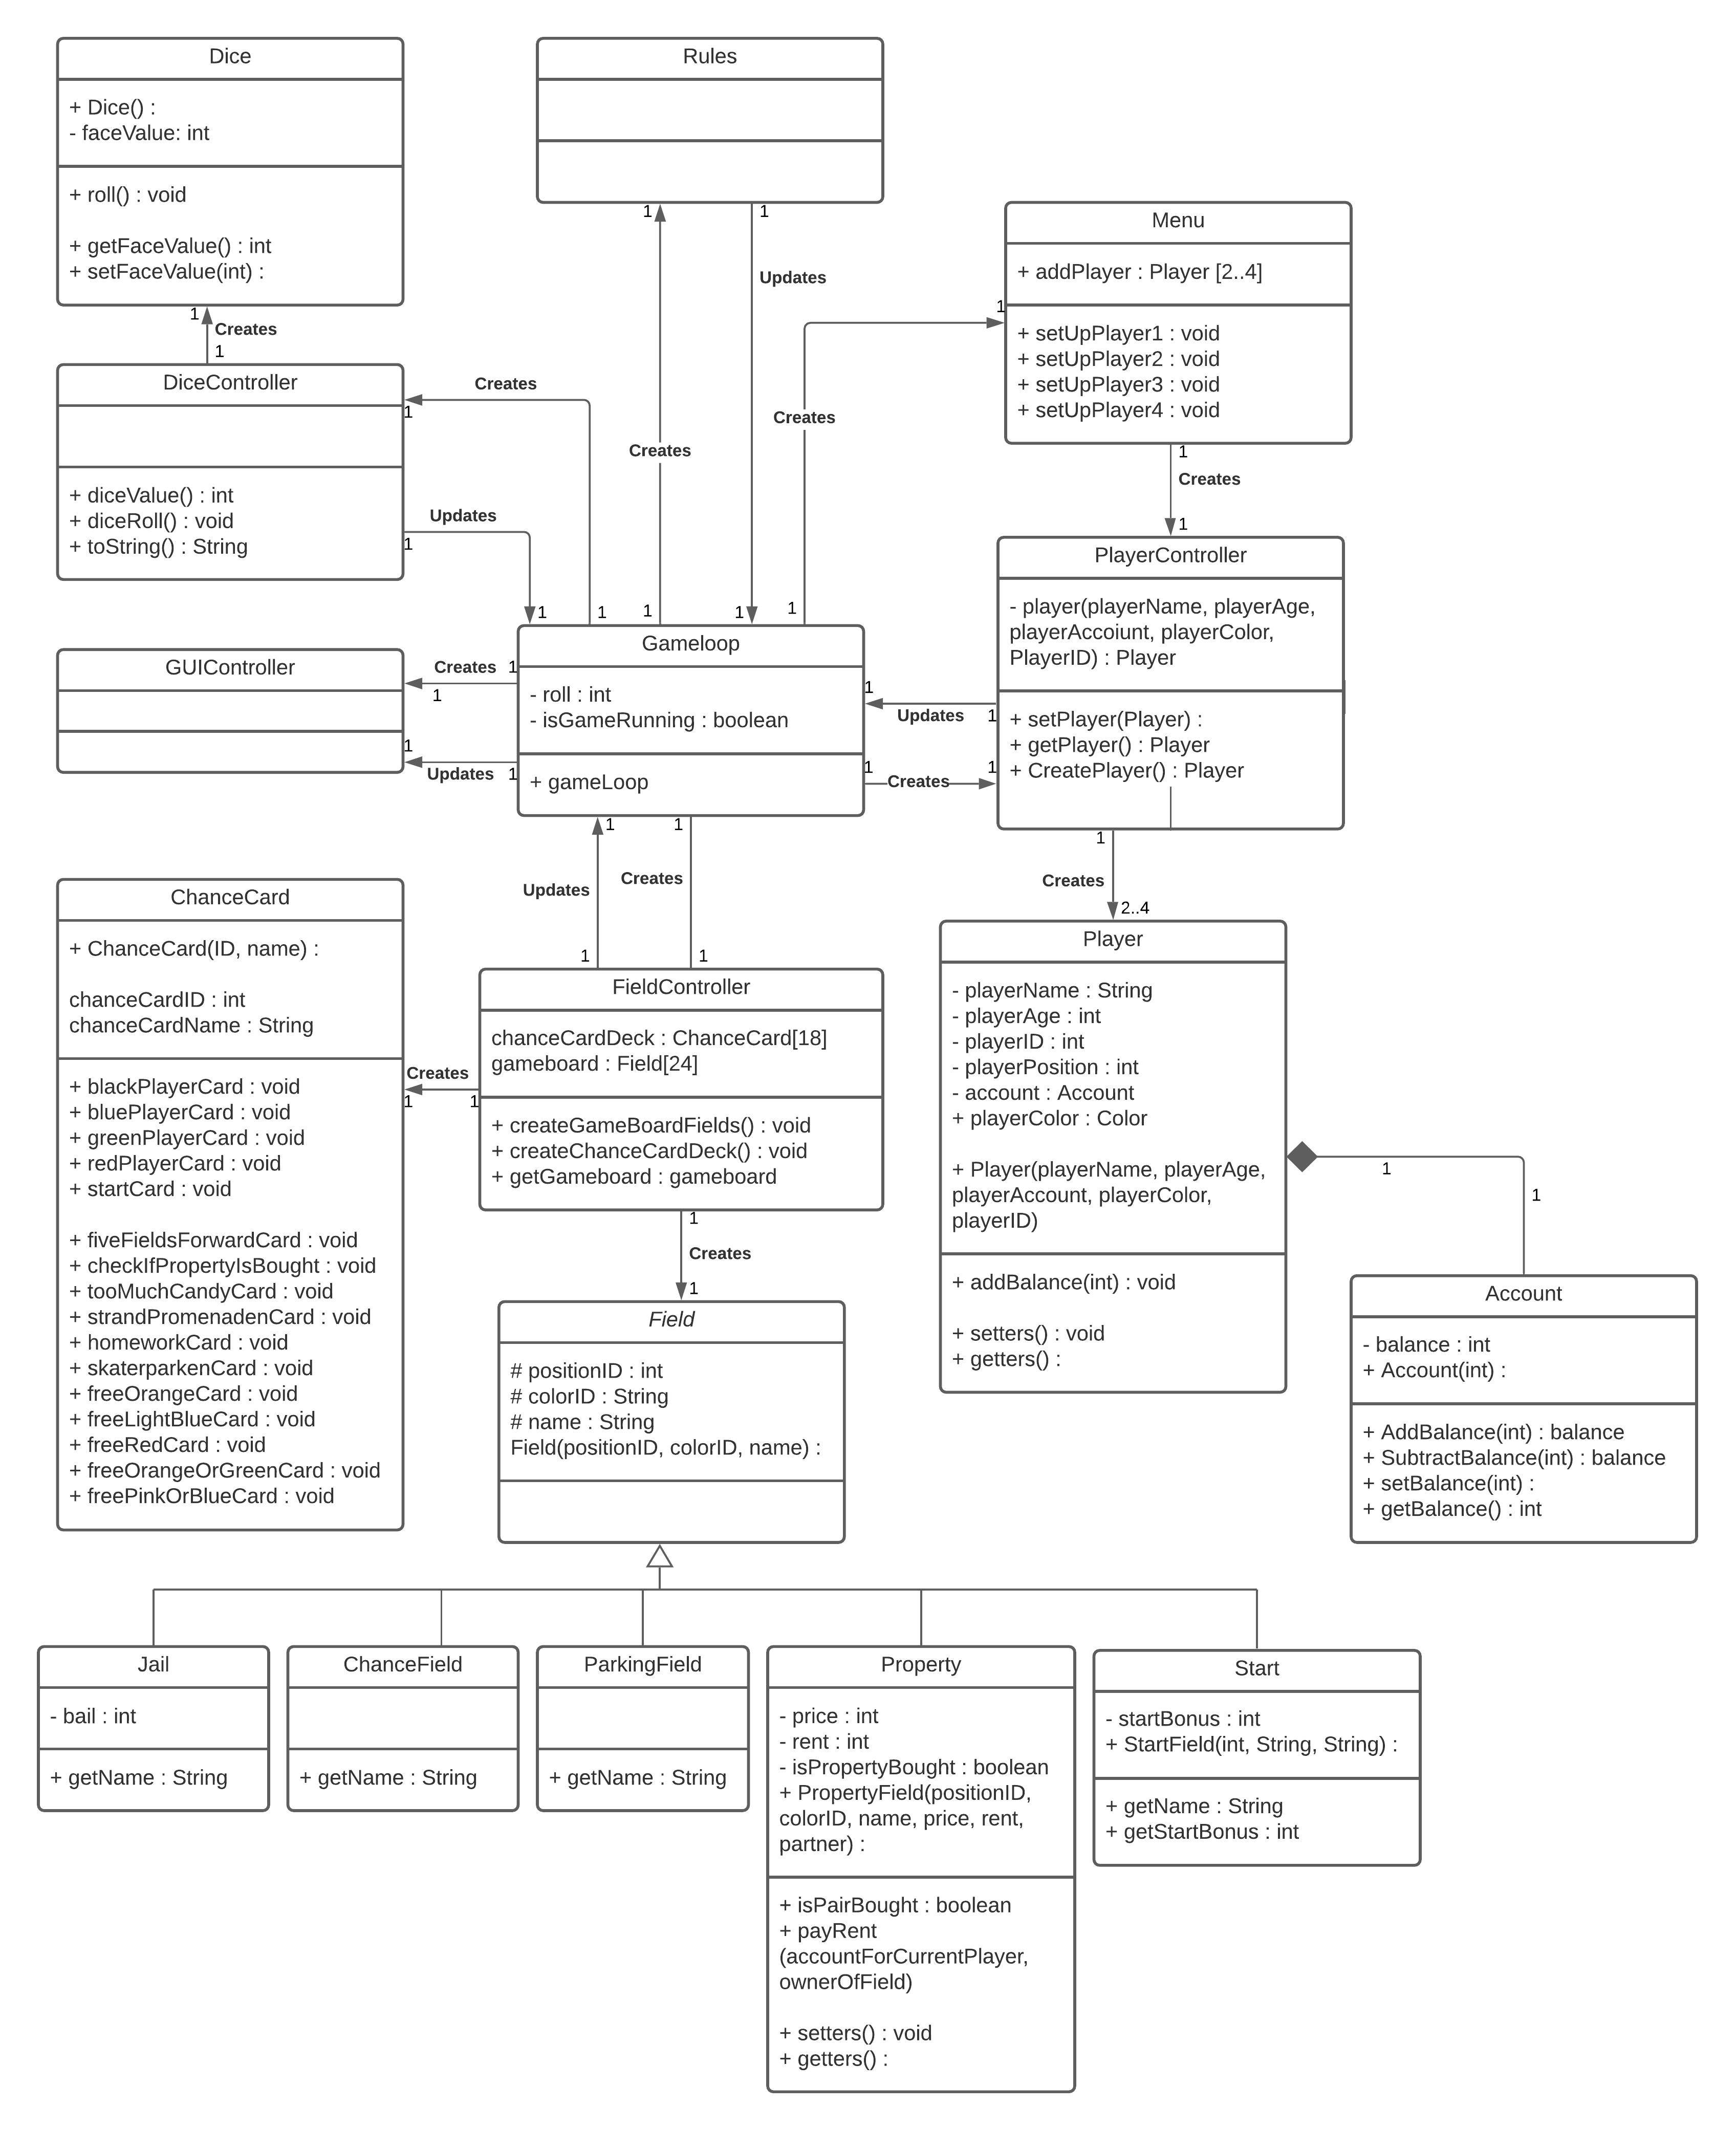
\includegraphics[width=0.9\textwidth]{Report/figures/Class Diagram.png}~\\[1cm]
\end{center}
Figur 5.2.1. Designklassediagram over Monopoly Junior spillet.
\end{flushleft}